% !Mode:: "TeX:UTF-8"
\documentclass{article}

%%%%%%%%------------------------------------------------------------------------
%%%% 日常所用宏包

%% 控制页边距
% 如果是beamer文档类, 则不用geometry
\makeatletter
\@ifclassloaded{beamer}{}{\usepackage[top=2.5cm, bottom=2.5cm, left=2.5cm, right=2.5cm]{geometry}}
\makeatother

%% 控制项目列表
\usepackage{enumerate}

%% 多栏显示
\usepackage{multicol}

%% 算法环境
\usepackage{algorithm}  
\usepackage{algorithmic} 
\usepackage{float} 

%% 网址引用
\usepackage{url}

%% 控制矩阵行距
\renewcommand\arraystretch{1.4}

%% hyperref宏包,生成可定位点击的超链接,并且会生成pdf书签
\makeatletter
\@ifclassloaded{beamer}{
\usepackage{hyperref}
}{
\usepackage[%
    pdfstartview=FitH,%
    CJKbookmarks=true,%
    bookmarks=true,%
    bookmarksnumbered=true,%
    bookmarksopen=true,%
    colorlinks=true,%
    citecolor=blue,%
    linkcolor=blue,%
    anchorcolor=green,%
    urlcolor=blue%
]{hyperref}
}
\makeatother



\makeatletter % 如果是 beamer 不需要下面两个包
\@ifclassloaded{beamer}{

}{
%% 控制标题
\usepackage{titlesec}
%% 控制目录
\usepackage{titletoc}
}
\makeatother

%% 控制表格样式
\usepackage{booktabs}

%% 控制字体大小
\usepackage{type1cm}

%% 首行缩进,用\noindent取消某段缩进
\usepackage{indentfirst}

%% 支持彩色文本、底色、文本框等
\usepackage{color,xcolor}

%% AMS LaTeX宏包: http://zzg34b.w3.c361.com/package/maths.htm#amssymb
\usepackage{amsmath,amssymb}

%%%% 基本插图方法
%% 图形宏包
\usepackage{graphicx}

%% 多个图形并排
\usepackage{subfig}

%%%% 基本插图方法结束

%%%% pgf/tikz绘图宏包设置
\usepackage{pgf,tikz}
\usetikzlibrary{shapes,automata,snakes,backgrounds,arrows}
\usetikzlibrary{mindmap}
%% 可以直接在latex文档中使用graphviz/dot语言,
%% 也可以用dot2tex工具将dot文件转换成tex文件再include进来
%% \usepackage[shell,pgf,outputdir={docgraphs/}]{dot2texi}
%%%% pgf/tikz设置结束


\makeatletter % 如果是 beamer 不需要下面两个包
\@ifclassloaded{beamer}{

}{
%%%% fancyhdr设置页眉页脚
%% 页眉页脚宏包
\usepackage{fancyhdr}
%% 页眉页脚风格
\pagestyle{plain}
}

%% 有时会出现\headheight too small的warning
\setlength{\headheight}{15pt}

%% 清空当前页眉页脚的默认设置
%\fancyhf{}
%%%% fancyhdr设置结束


\makeatletter % 对 beamer 要重新设置
\@ifclassloaded{beamer}{

}{
%%%% 设置listings宏包用来粘贴源代码
%% 方便粘贴源代码,部分代码高亮功能
\usepackage{listings}

%% 设置listings宏包的一些全局样式
%% 参考http://hi.baidu.com/shawpinlee/blog/item/9ec431cbae28e41cbe09e6e4.html
\lstset{
showstringspaces=false,              %% 设定是否显示代码之间的空格符号
numbers=left,                        %% 在左边显示行号
numberstyle=\tiny,                   %% 设定行号字体的大小
basicstyle=\footnotesize,                    %% 设定字体大小\tiny, \small, \Large等等
keywordstyle=\color{blue!70}, commentstyle=\color{red!50!green!50!blue!50},
                                     %% 关键字高亮
frame=shadowbox,                     %% 给代码加框
rulesepcolor=\color{red!20!green!20!blue!20},
escapechar=`,                        %% 中文逃逸字符,用于中英混排
xleftmargin=2em,xrightmargin=2em, aboveskip=1em,
breaklines,                          %% 这条命令可以让LaTeX自动将长的代码行换行排版
extendedchars=false                  %% 这一条命令可以解决代码跨页时,章节标题,页眉等汉字不显示的问题
}}
\makeatother
%%%% listings宏包设置结束


%%%% 附录设置
\makeatletter % 对 beamer 要重新设置
\@ifclassloaded{beamer}{

}{
\usepackage[title,titletoc,header]{appendix}
}
\makeatother
%%%% 附录设置结束


%%%% 日常宏包设置结束
%%%%%%%%------------------------------------------------------------------------


%%%%%%%%------------------------------------------------------------------------
%%%% 英文字体设置结束
%% 这里可以加入自己的英文字体设置
%%%%%%%%------------------------------------------------------------------------

%%%%%%%%------------------------------------------------------------------------
%%%% 设置常用字体字号,与MS Word相对应

%% 一号, 1.4倍行距
\newcommand{\yihao}{\fontsize{26pt}{36pt}\selectfont}
%% 二号, 1.25倍行距
\newcommand{\erhao}{\fontsize{22pt}{28pt}\selectfont}
%% 小二, 单倍行距
\newcommand{\xiaoer}{\fontsize{18pt}{18pt}\selectfont}
%% 三号, 1.5倍行距
\newcommand{\sanhao}{\fontsize{16pt}{24pt}\selectfont}
%% 小三, 1.5倍行距
\newcommand{\xiaosan}{\fontsize{15pt}{22pt}\selectfont}
%% 四号, 1.5倍行距
\newcommand{\sihao}{\fontsize{14pt}{21pt}\selectfont}
%% 半四, 1.5倍行距
\newcommand{\bansi}{\fontsize{13pt}{19.5pt}\selectfont}
%% 小四, 1.5倍行距
\newcommand{\xiaosi}{\fontsize{12pt}{18pt}\selectfont}
%% 大五, 单倍行距
\newcommand{\dawu}{\fontsize{11pt}{11pt}\selectfont}
%% 五号, 单倍行距
\newcommand{\wuhao}{\fontsize{10.5pt}{10.5pt}\selectfont}
%%%%%%%%------------------------------------------------------------------------


%% 设定段间距
\setlength{\parskip}{0.5\baselineskip}

%% 设定行距
\linespread{1}


%% 设定正文字体大小
 \renewcommand{\normalsize}{\sihao}

%制作水印
\RequirePackage{draftcopy}
\draftcopyName{XTUMESH}{100}
\draftcopySetGrey{0.90}
\draftcopyPageTransform{40 rotate}
\draftcopyPageX{350}
\draftcopyPageY{80}

%%%% 个性设置结束
%%%%%%%%------------------------------------------------------------------------


%%%%%%%%------------------------------------------------------------------------
%%%% bibtex设置

%% 设定参考文献显示风格
% 下面是几种常见的样式
% * plain: 按字母的顺序排列,比较次序为作者、年度和标题
% * unsrt: 样式同plain,只是按照引用的先后排序
% * alpha: 用作者名首字母+年份后两位作标号,以字母顺序排序
% * abbrv: 类似plain,将月份全拼改为缩写,更显紧凑
% * apalike: 美国心理学学会期刊样式, 引用样式 [Tailper and Zang, 2006]

\makeatletter
\@ifclassloaded{beamer}{
\bibliographystyle{apalike}
}{
\bibliographystyle{unsrt}
}
\makeatother


%%%% bibtex设置结束
%%%%%%%%------------------------------------------------------------------------

%%%%%%%%------------------------------------------------------------------------
%%%% xeCJK相关宏包

\usepackage{xltxtra,fontspec,xunicode}
\usepackage[slantfont, boldfont]{xeCJK} 
\usepackage{subfig}

%% 针对中文进行断行
\XeTeXlinebreaklocale "zh"             

%% 给予TeX断行一定自由度
\XeTeXlinebreakskip = 0pt plus 1pt minus 0.1pt

%%%% xeCJK设置结束                                       
%%%%%%%%------------------------------------------------------------------------

%%%%%%%%------------------------------------------------------------------------
%%%% xeCJK字体设置

%% 设置中文标点样式,支持quanjiao、banjiao、kaiming等多种方式
\punctstyle{kaiming}                                        
                                                     
%% 设置缺省中文字体
\setCJKmainfont[BoldFont={Adobe Heiti Std}, ItalicFont={Adobe Kaiti Std}]{Adobe Song Std}   
%% 设置中文无衬线字体
\setCJKsansfont[BoldFont={Adobe Heiti Std}]{Adobe Kaiti Std}  
%% 设置等宽字体
\setCJKmonofont{Adobe Heiti Std}                            

%% 英文衬线字体
\setmainfont{DejaVu Serif}                                  
%% 英文等宽字体
\setmonofont{DejaVu Sans Mono}                              
%% 英文无衬线字体
\setsansfont{DejaVu Sans}                                   

%% 定义新字体
\setCJKfamilyfont{song}{Adobe Song Std}                     
\setCJKfamilyfont{kai}{Adobe Kaiti Std}
\setCJKfamilyfont{hei}{Adobe Heiti Std}
\setCJKfamilyfont{fangsong}{Adobe Fangsong Std}
\setCJKfamilyfont{lisu}{LiSu}
\setCJKfamilyfont{youyuan}{YouYuan}

%% 自定义宋体
\newcommand{\song}{\CJKfamily{song}}                       
%% 自定义楷体
\newcommand{\kai}{\CJKfamily{kai}}                         
%% 自定义黑体
\newcommand{\hei}{\CJKfamily{hei}}                         
%% 自定义仿宋体
\newcommand{\fangsong}{\CJKfamily{fangsong}}               
%% 自定义隶书
\newcommand{\lisu}{\CJKfamily{lisu}}                       
%% 自定义幼圆
\newcommand{\youyuan}{\CJKfamily{youyuan}}                 

%%%% xeCJK字体设置结束
%%%%%%%%------------------------------------------------------------------------

%%%%%%%%------------------------------------------------------------------------
%%%% 一些关于中文文档的重定义
\newcommand{\chntoday}{\number\year\,年\,\number\month\,月\,\number\day\,日}
%% 数学公式定理的重定义

%% 中文破折号,据说来自清华模板
\newcommand{\pozhehao}{\kern0.3ex\rule[0.8ex]{2em}{0.1ex}\kern0.3ex}

\newtheorem{example}{例}                                   
\newtheorem{theorem}{定理}[section]                         
\newtheorem{definition}{定义}
\newtheorem{axiom}{公理}
\newtheorem{property}{性质}
\newtheorem{proposition}{命题}
\newtheorem{lemma}{引理}
\newtheorem{corollary}{推论}
\newtheorem{remark}{注解}
\newtheorem{condition}{条件}
\newtheorem{conclusion}{结论}
\newtheorem{assumption}{假设}

\makeatletter %
\@ifclassloaded{beamer}{

}{
%% 章节等名称重定义
\renewcommand{\contentsname}{目录}     
\renewcommand{\indexname}{索引}
\renewcommand{\listfigurename}{插图目录}
\renewcommand{\listtablename}{表格目录}
\renewcommand{\appendixname}{附录}
\renewcommand{\appendixpagename}{附录}
\renewcommand{\appendixtocname}{附录}
%% 设置chapter、section与subsection的格式
\titleformat{\chapter}{\centering\huge}{第\thechapter{}章}{1em}{\textbf}
\titleformat{\section}{\centering\sihao}{\thesection}{1em}{\textbf}
\titleformat{\subsection}{\xiaosi}{\thesubsection}{1em}{\textbf}
\titleformat{\subsubsection}{\xiaosi}{\thesubsubsection}{1em}{\textbf}

\@ifclassloaded{book}{

}{
\renewcommand{\abstractname}{摘要}
}
}
\makeatother

\renewcommand{\figurename}{图}
\renewcommand{\tablename}{表}

\makeatletter
\@ifclassloaded{book}{
\renewcommand{\bibname}{参考文献}
}{
\renewcommand{\refname}{参考文献} 
}
\makeatother

\floatname{algorithm}{算法}
\renewcommand{\algorithmicrequire}{\textbf{输入:}}
\renewcommand{\algorithmicensure}{\textbf{输出:}}

%%%% 中文重定义结束
%%%%%%%%------------------------------------------------------------------------

\setCJKmainfont{STKaiti} % 如果请替换为本地系统有的字体
%中文断行
\XeTeXlinebreaklocale "zh"
\XeTeXlinebreakskip = 16pt plus 16pt 
\begin{document}
\title{曲面有限元及其应用}
\author{刘江刚 \ \ 龚欣}
\date{\today}
\maketitle
%\tableofcontents
\newpage
\section{基础知识}
\subsection{梯度}
首先给出梯度的概念,它是由数量函数$u(x,y,z)$所定义的向量函数
\begin{equation*}
\text{grad}~u=\left(\frac{\partial u}{\partial x},\frac{\partial u}{\partial y},\frac{\partial u}{\partial z}\right) 
\end{equation*}
而且$\text{grad}~u$的方向就是使$\frac{\partial u}{\partial l}$达到最大值的方向,它的大小就是$u$在这个方向上的方向导数.

引进符号向量
\begin{equation*}
\nabla=\left(\frac{\partial}{\partial x},\frac{\partial}{\partial y},\frac{\partial}{\partial z}\right)
\end{equation*}
当把它作为运算符号来看待时,梯度可写作
\begin{equation*}
\text{grad}~u=\nabla u
\end{equation*}

关于梯度,有以下一些基本性质:

1.若$u,v$是数量函数,则
\begin{equation*}
\nabla(u+v)=\nabla u+\nabla v
\end{equation*}

2.若$u,v$是数量函数,则
\begin{equation*}
\nabla(uv)=u(\nabla v)+v(\nabla u)
\end{equation*}

3.若$u(x,y,z)$是数量函数,则$\nabla^2u(x)\in R^{3\times 3}$为$u(x)$的Hessian矩阵
\begin{equation*}
\nabla^2u(x)=
\begin{pmatrix}
\frac{\partial^2u}{\partial x^2} & \frac{\partial^2u}{\partial x\partial y} & \frac{\partial^2u}{\partial x\partial z} \\
\frac{\partial^2u}{\partial y\partial x} & \frac{\partial^2u}{\partial y^2} & \frac{\partial^2u}{\partial y\partial z} \\
\frac{\partial^2u}{\partial z\partial x} & \frac{\partial^2u}{\partial z\partial y} & \frac{\partial^2u}{\partial z^2} 
\end{pmatrix}
\end{equation*}
\subsection{散度}
设
\begin{equation*}
\boldsymbol{A}(x,y,z)=(P(x,y,z),Q(x,y,z),R(x,y,z))
\end{equation*}
为空间区域$V$上的向量函数,对$V$上每一点$(x,y,z)$,定义数量函数
\begin{equation*}
D(x,y,z)=\frac{\partial P}{\partial x}+\frac{\partial Q}{\partial y}+\frac{\partial R}{\partial z}
\end{equation*}
称它为向量函数$\boldsymbol{A}$在$(x,y,z)$处的散度,记作
\begin{equation*}
D(x,y,z)=\text{div}~\boldsymbol{A}(x,y,z)
\end{equation*}

由前面引进的算符$\nabla$,$\boldsymbol{A}$的散度的向量形式是
\begin{equation*}
\text{div}~\boldsymbol{A}=\nabla\cdot\boldsymbol{A}
\end{equation*}
关于散度,有以下一些基本性质:

1.若$\boldsymbol{u},\boldsymbol{v}$是向量函数,则
\begin{equation*}
\nabla\cdot(\boldsymbol{u}+\boldsymbol{v})=\nabla\cdot\boldsymbol{u}+\nabla\cdot\boldsymbol{v}
\end{equation*}

2.若$\varphi$是数量函数,$\boldsymbol{F}$是向量函数,则
\begin{equation*}
\nabla\cdot(\varphi\boldsymbol{F})=\varphi\nabla\cdot\boldsymbol{F}+F\cdot\nabla\varphi
\end{equation*}

3.若$\varphi=\varphi(x,y,z)$是一数量函数,则
\begin{equation*}
\nabla\cdot\nabla\varphi=\frac{\partial^2\varphi}{\partial x^2}+\frac{\partial^2\varphi}{\partial y^2}+\frac{\partial^2\varphi}{\partial z^2}
\end{equation*}
算符$\nabla$的内积$\nabla\cdot\nabla$常记作$\Delta$,于是有
\begin{equation*}
\nabla\cdot\nabla\varphi=\Delta\varphi
\end{equation*}
\section{预备知识}
\subsection{连续的曲面$S$}
设$S$是一个闭曲面,所以$\partial S=\varnothing$,所以$S$把$\mathbb{R}^3$分成三个不同的集合:曲面内部的点、曲面上的点和曲面外部的点,分别表示为$\Omega_{-}$、$\Omega_0$和$\Omega_{+}$.对于任意的$x\in\mathbb{R}^3$,记$\mathrm{dist}(x,S)=\min\limits_{y\in S}\left|x-y\right|$为$x$和$S$之间的距离,其中$|\cdot|$为标准的欧氏距离.我们可以定义一个带状区域:$U:=\left\{x\in\mathbb{R}^3|\mathrm{dist}(x,S)<\delta\right\}$,其中$\delta>0$且要足够小,使得可以定义一个唯一的符号距离函数$d:U\rightarrow\mathbb{R}$,满足如下性质:
\begin{equation}\label{eq:MA}
\left\{
\begin{array}{l}
d\in C^3(U),\\
|d(x)|=\mathrm{dist}(x,S),\quad \forall x\in U,\\
d(x)< 0,\quad\forall x\in\Omega_{-}\cap U,\\
d(x)= 0,\quad\forall x\in \Omega_0\cap U,\\
d(x)> 0,\quad\forall x\in\Omega_{+}\cap U,\\
\end{array}\right.
\end{equation}
对于任意的$x\in U$,可视$S$为符号距离函数的零水平集.

记$\nabla$为$\mathbb{R}^3$中通常意义下的梯度算子,$\nabla d(x)\in\mathbb{R}^3$为$d(x)$的梯度,$\boldsymbol{H}(x):=\nabla^2d(x)\in\mathbb{R}^{3\times 3}$为$d(x)$的Hessian矩阵.对于任意的$x\in U$,记$y$为$S$上离$x$最近的点,也即$|d(x)|=\left|x-y\right|$.因为$d(x)$是符号距离函数,且$S$是它的零水平集,易知$\nabla d(x)$是$S$在$y$处的单位外法向向量,即$\left|\nabla d(x)\right|=1$.对于任意的$x\in U$,记$\boldsymbol{n}(x)=\nabla d(x)$,我们可以定义如下唯一的投影
$\mathcal{P}_0:U\rightarrow S$:
\begin{equation*}
\mathcal{P}_0(x):=x-d(x)\boldsymbol{n}(x)\quad(1)
\end{equation*}
对于$v\in C^1(S)$,因为$S$是$C^3$的,我们可以把$v$扩展到$C^1(U)$,且仍记为$v$.定义$v$在$S$上的切向梯度为
\begin{equation*}
\nabla_Sv=\nabla v-(\nabla v\cdot\boldsymbol{n})\boldsymbol{n}=(I-\boldsymbol{n}\boldsymbol{n}^t)\nabla v=\boldsymbol{P}\nabla v\in\mathbb{R}^3
\end{equation*}
其中$\boldsymbol{P}(x)=(I-\boldsymbol{n}\boldsymbol{n}^t)(x)$是到点$x\in S$切平面上的投影算子,因此有$\boldsymbol{P}^2=\boldsymbol{P}$.注意到这里我们用$v$的扩展来定义曲面梯度.然而,可以证明$\nabla_Sv$的定义只依赖$v$的$S$上的值而不是$v$的扩展,也即$\nabla_S$是一个内蕴算子.

类似地,对于一个向量场$\boldsymbol{v}\in(C^1(S))^3$,我们也可以把它扩展到$(C^1(U))^3$上去,并定义$\boldsymbol{v}$在$S$上的切向散度为
\begin{equation*}
\nabla_S\cdot\boldsymbol{v}=\nabla\cdot\boldsymbol{v}-\boldsymbol{n}^t\nabla\boldsymbol{v}\boldsymbol{n}\in\mathbb{R}
\end{equation*}

曲面S上的Laplace-Beltrami算子定义如下:
\begin{equation*}
\Delta_Sv=\nabla_S\cdot(\nabla_Sv)=\Delta v-(\nabla v\cdot\boldsymbol{n})(\nabla\cdot\boldsymbol{n})-\boldsymbol{n}^t\nabla^2v\boldsymbol{n}\in\mathbb{R}
\end{equation*}
其中$v\in C^2(S)$,$\nabla^2v$是$v$的Hessian矩阵(扩展为$C^2(U)$函数)
\subsection{离散的曲面$S_h$和网格$\mathcal{T}_h$}
\begin{figure}[H]
\centering
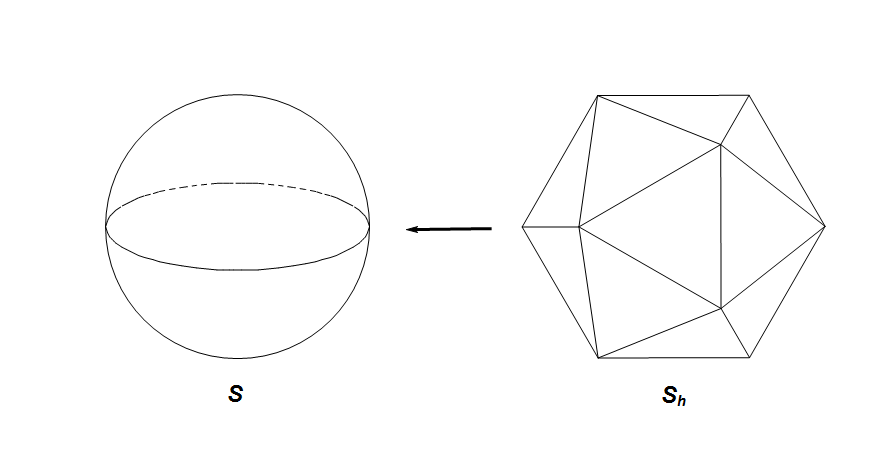
\includegraphics[scale=0.5]{./figures/picture_1.png}
\caption{}
\end{figure}
记$S_h\subset U$是由三角形单元$\tau_h$组成的多面体面,即$S_h$逼近曲面$S$,我们假设$S_h$的这些三角形单元是正则的,单元尺寸是拟一致的,且它们的顶点都在曲面$S$上.其中$\mathcal{N}_h=\left\{x_i\right\}$为$S_h$所有顶点的集合,$\mathcal{T}_h=\left\{\tau_h\right\}$ 为所有三角形单元的集合,$\mathcal{E}_h=\left\{E\right\}$为所有边的集合.对于任意的$\tau_h\in\mathcal{T}_h$,记$\boldsymbol{n}_h$为$S_h$在$\tau_h$上的单位外法向向量.对于$v_h\in C(S_h)$和$v_h|_{\tau_h}$,我们有
\begin{equation*}
\nabla_{S_h}v_h|_{\tau_h}:=\nabla v_h-(\nabla v_h\cdot\boldsymbol{n}_h)\boldsymbol{n}_h=(\boldsymbol{I}-\boldsymbol{n}_h\boldsymbol{n}^t_h)\nabla v_h=\boldsymbol{P}_h\nabla v_h\in\mathbb{R}^3
\end{equation*}
其中$\boldsymbol{P}_h=\boldsymbol{I}-\boldsymbol{n}_h\boldsymbol{n}^t_h\in\mathbb{R}^{3\times 3}$.显然$\nabla_{S_h}v_h\in(L^2(S_h))^3$

如果限制投影$\mathcal{P}_0:U\rightarrow S$到$S_h$上,就得到一个从$S_h$到$S$的连续可微的双射,仍记为$\mathcal{P}_0$.对于任意的$\tau_h\in\mathcal{T}_h$,我们可以得到一个曲面三角形$\tau:=\mathcal{P}_0(\tau_h)$,并记所有的曲面三角形集合为$\mathcal{T}_S$.

下面我们建立定义在$S$和$S_h$函数之间的关系.借助双射投影$\mathcal{P}_0$,可以由函数$v:S\rightarrow\mathbb{R}$唯一地引入另一个函数$\bar{v}:S_h\rightarrow\mathbb{R}$.对于所有的$x\in S_h$,有$\bar{v}(x)=v(\mathcal{P}_0(x))$.对于任意的$\tau_h\in\mathcal{T}_h$和函数$v\in C^1(\mathcal{P}_0(\tau_h))$,我们有
\begin{equation*}
\nabla_{S_h}\bar{v}(x)=(\boldsymbol{P}_h(\boldsymbol{I}-d\boldsymbol{H})\boldsymbol{P})(x)\nabla_{S}v(\mathcal{P}_0(x))\quad\forall x\in \tau_h.
\end{equation*}
反过来,一个函数$v_h:S_h\rightarrow\mathbb{R}$也可以唯一的引入一个函数$\tilde{v}_h:S\rightarrow\mathbb{R}$,对于所有的$x\in S$,有$\tilde{v}_h(x)=v_h(\mathcal{P}^{-1}_0(x))$.对于任意的$\tau_h\in\mathcal{T}_h$和函数$v_h\in C^1(\tau_h)$让$\tau=\mathcal{P}_0(\tau_h)$,可得
\begin{equation*}
\nabla_{S}\tilde{v}_h(x)=(\boldsymbol{I}-d\boldsymbol{H})^{-1}\left(\boldsymbol{I}-\frac{\boldsymbol{n}_h\boldsymbol{n}^t}{\boldsymbol{n}^t\boldsymbol{n}_h}\right)\nabla_{S_h}v_h(\mathcal{P}^{-1}_0(x))\quad\forall x\in\tau.
\end{equation*}

\section{曲面线性有限元}

对于三角形$\tau_h\in\mathcal{T}_h$, 记$\{\lambda_i\}$为$\tau_h$的重心坐标.   
记$\mathcal V_h$为$S_h$上的连续分片线性有限元空间, 也即对于任意的$v_h\in \mathcal V_h$和$\tau_h \in \mathcal T_h$,
$v_h$在$S_h$上连续, 且有$v_h|_{\tau_h}\in {\rm span}\{\lambda_1,\lambda_2,\lambda_3\}$.  
我们可定义$S$上的提升空间
\begin{eqnarray*}
 \tilde{V}_{h} & = &
\{\tilde{v}_{h} \, | \, \tilde{v}_{h}:=v_{h}\circ\mathcal{P}_{0}^{-1},\,
\text{其中 }v_{h}\in \mathcal V_h\},
\end{eqnarray*}
其中$\mathcal P_0: S_h \to S$为定义在(1)中的双射.   
对于$f\in L^{2}(S)$, 记
\begin{equation}\label{eq:fh}
f_{h}(x)=\bar{f}(x)-\frac{1}{|S_{h}|}\int_{S_{h}} \bar f \, \mathrm{d}\sigma_{h},
\end{equation}
其中$|S_{h}|$ 为 $ S_{h}$的总面积. 那么有
$\int_{S_{h}}f_{h}(x)\,\mathrm{d}\sigma_{h}=0$, 且下列方程存在唯一的有限元解
$u_{h}\in \mathcal V_h$, 满足$\int_{S_{h}}u_{h}\,\mathrm{d}\sigma_{h}=0$
\begin{equation*}
\int_{S_h}\nabla_{S_h}u_h\cdot\nabla_{S_h}v_h\mathrm{d}\sigma_h=\int_{S_h}f_hv_h\mathrm{d}\sigma_h\quad\forall v_h\in\mathcal{V}_h
\end{equation*}

\section{曲面高次元}
\subsection{符号说明}
\begin{table}[H]
\begin{center}
\begin{tabular}{|c|c|}
 \hline
 $S$  &$\mathbb R^3$ 空间中的曲面\\
 \hline
 $K\subset \mathbb R^2$  &二维空间中的标准单元\\
 \hline
 $\mathbf u = (u, v)^T$  &二维空间中的坐标系\\
 \hline
 $\tau_h \subset R^3$  &三维空间中的尺寸为 $h$ 的平面三角形\\  
 \hline
 $\mathbf x = (x, y, z)^T\in \tau_h$  &$\tau_h$ 上的一个点\\
 \hline
 $\mathcal P_0$  &$S$ 邻近区域到 $S$ 的投影\\
 \hline
 $\mathbf x_i,  i=1,\cdots, n_{dof}$  &$\tau_h$ 上 $p$ 次 Lagrangian 基函数对应的自由度坐标点\\
 \hline
 $\tau_p\subset \mathbb R^3$ &定义在 $\tau_h$ 上的 $p$ 次多项式曲面三角形\\
 \hline
 $ \mathbf x_p =(x_p, y_p, z_p)^T \in \tau_p$ & $\tau_p$ 上一个点的三维坐标\\
 \hline
 $\tau_S\subset \mathbb R^3$ & 把 $\tau_h$ 投影到曲面 $S$ 上的曲面三角形\\
 \hline
 $ \mathbf x_S =(x_S, y_S, z_S)^T \in \tau_S$ & $\tau_S$ 上一个点的三维坐标 \\
 \hline
 $\varphi_i(\mathbf x)$ & 定义在 $\tau_h$ 上第 $i$ 个 Lagrangian 基函数\\
 \hline 
\end{tabular}
\end{center}
\end{table}

\subsection{$\tau_h$$\quad$$\tau_p$和$\tau_s$之间关系}

对于 $\tau_p$ 上的任意一点 $\mathbf x_p$, 存在一点 $\mathbf x \in \tau_h$, 使得
\begin{equation*}
\mathbf x_p = \sum_{i=1}^{n_{dof}} \mathbf x_i \varphi_i(\mathbf x)
\end{equation*}
进一步, 存在标准参考单元 $K$ 中存在一点 $\mathbf u = (u,v)$, 可得
\begin{equation*}
\mathbf x(u,v) = \lambda_0 \mathbf x_0 + \lambda_1 \mathbf x_1 + \lambda_2 \mathbf x_2
\end{equation*}
其中 $\mathbf x_0$, $\mathbf x_1$ 和 $\mathbf x_2$ 为$\tau_h$ 的三个顶点, 
\begin{equation*}
\lambda_0 = 1- u - v,\quad\lambda_1 = u,\quad\lambda_2 = v
\end{equation*}
对于 $\tau_S$ 上的任意一点 $\mathbf x_S$, 存在 $\tau_p$ 上的一点 $\mathbf x_p$, 使得
\begin{equation*}
\mathbf x_S = \mathcal P_0(\mathbf x_p)
\end{equation*}
$\mathbf x$ 关于  $(u, v)$ 的 Jacobi 矩阵为
\begin{equation*}
\frac{\partial \mathbf x}{\partial \mathbf u} = [\mathbf x_1 - \mathbf x_0, \mathbf x_2 - \mathbf x_0]
\end{equation*}
$\mathbf x_p$ 关于 $\mathbf x$ 的 Jacobi 矩阵为
\begin{equation*}
\frac{\partial \mathbf x_p}{\partial \mathbf x} = \sum_{i=1}^{n_{dof}}
\begin{bmatrix}
x_i\nabla_{\mathbf x}\varphi_i(\mathbf x)^T\\
y_i\nabla_{\mathbf x}\varphi_i(\mathbf x)^T\\
z_i\nabla_{\mathbf x}\varphi_i(\mathbf x)^T\\
\end{bmatrix}
\end{equation*}
则 $\mathbf x_p$ 关于 $\mathbf u$ 的 Jacobi 矩阵为
\begin{equation*}
\frac{\partial \mathbf x_p}{\partial \mathbf u}=[\frac{\partial \mathbf x_p}{\partial u}, \frac{\partial \mathbf x_p}{\partial v}]=\sum_{i=1}^{n_{dof}}
\begin{bmatrix}
x_i\nabla_{\mathbf x}\varphi_i(\mathbf x)^T\\
y_i\nabla_{\mathbf x}\varphi_i(\mathbf x)^T\\
z_i\nabla_{\mathbf x}\varphi_i(\mathbf x)^T\\
\end{bmatrix}
[\mathbf x_1 - \mathbf x_0, \mathbf x_2 - \mathbf x_0]\qquad(2)
\end{equation*}
记
\begin{equation*} 
\mathrm d \mathbf x_p = \frac{\partial \mathbf x_p}{\partial \mathbf u}\mathrm d \mathbf u = \frac{\partial \mathbf x_p}{\partial u}\mathrm d u + \frac{\partial \mathbf x_p}{\partial v}\mathrm d v,
\end{equation*}
其中 $\mathrm d \mathbf u = [\mathrm d u, \mathrm d v]^T$.
进一步可得曲面三角形 $\tau_p$ 上的第一基本形式
\begin{equation*}
I = <\mathrm d \mathbf x_p, \mathrm d \mathbf x_p> = \mathrm d \mathbf u^T 
\begin{bmatrix}
g_{11} & g_{12}\\
g_{12} & g_{22}
\end{bmatrix}
\mathrm d \mathbf u
\end{equation*}
其中 
\begin{equation*}
g_{11} =<\frac{\partial \mathbf x_p}{\partial u}, \frac{\partial \mathbf x_p}{\partial u}>, 
g_{12} =<\frac{\partial \mathbf x_p}{\partial u}, \frac{\partial \mathbf x_p}{\partial v}>, 
g_{22} =<\frac{\partial \mathbf x_p}{\partial v}, \frac{\partial \mathbf x_p}{\partial v}>, 
\end{equation*}
定义$\tau_p$ 上的基函数如下
\begin{equation*}
\varphi_{p,i}(\mathbf x_p) =\varphi_i(\mathbf x) 
\end{equation*}
其中
\begin{equation*}
\mathbf x_p = \sum_{i=1}^{n_{dof}} \mathbf x_i \varphi_i(\mathbf x)
\end{equation*}
则 $\varphi_{p,i}(\mathbf x_p)$ 在 $\tau_p$ 上的切向导数定义如下:
\begin{equation*}
\nabla_{S_p} \varphi_{p,i} = \frac{\partial \mathbf x_p}{\partial \mathbf u}\begin{bmatrix}
g_{11} & g_{12}\\
g_{12} & g_{22}
\end{bmatrix}^{-1}(\frac{\partial \mathbf x}{\partial \mathbf u})^T\nabla_{S_h}\varphi_i(\mathbf x)
\end{equation*}

\subsection{$S$上曲面三角形的面积计算公式}

\begin{equation*}
\mathcal P_0(\mathbf x):=\mathbf x - d(\mathbf x)\mathbf n(\mathbf x)
\end{equation*}
对于$\mathbf x_p \in \tau_p$, 存在 $\mathbf x_S \in S$, 有
\begin{equation*}
\mathbf x_S = \mathcal P_0(\mathbf x_p)=\mathbf x_p - d(\mathbf x_p)\mathbf n(\mathbf x_p)
\end{equation*}
\begin{equation*}
\frac{\partial \mathbf x_S}{\partial\mathbf x_p} = I - d(\mathbf x_p) H(\mathbf x_p) - \mathbf n(\mathbf x_p)\mathbf n(\mathbf x_p)^T
\end{equation*}
\begin{equation*}
\frac{\partial \mathbf x_S}{\partial\mathbf u} = \frac{\partial \mathbf x_S}{\partial\mathbf x_p}\frac{\partial \mathbf x_p}{\partial\mathbf u}
\end{equation*}

\subsection{$S$上的导数计算}

考虑 $\tau_S$ 和 $\tau_p$ 的关系

则 $\mathbf x_S$ 关于 $\mathbf u$ 的 Jacobi 矩阵为
\begin{equation*}
\frac{\partial \mathbf x_S}{\partial\mathbf u} = \frac{\partial \mathbf x_S}{\partial\mathbf x_p}\frac{\partial \mathbf x_p}{\partial\mathbf u}
\end{equation*}
\begin{equation*}
\frac{\partial \mathbf x_S}{\partial\mathbf x_p} = I - d(\mathbf x_p) H(\mathbf x_p) - \mathbf n(\mathbf x_p)\mathbf n(\mathbf x_p)^T
\end{equation*}
由于
\begin{equation*}
\frac{\partial \mathbf x_p}{\partial \mathbf u}=[\frac{\partial \mathbf x_p}{\partial u}, \frac{\partial \mathbf x_p}{\partial v}]=\sum_{i=1}^{n_{dof}}
\begin{bmatrix}
x_i\nabla_{\mathbf x}\varphi_i(\mathbf x)^T\\
y_i\nabla_{\mathbf x}\varphi_i(\mathbf x)^T\\
z_i\nabla_{\mathbf x}\varphi_i(\mathbf x)^T\\
\end{bmatrix}
[\mathbf x_1 - \mathbf x_0, \mathbf x_2 - \mathbf x_0]
\end{equation*}
即,很容易计算
\begin{equation*}
\frac{\partial \mathbf x_S}{\partial\mathbf u}
\end{equation*}
进一步可得到曲面 $\tau_S$ 上的第一基本形式
记
\begin{equation*} 
\mathrm d \mathbf x_S = \frac{\partial \mathbf x_S}{\partial \mathbf u}\mathrm d \mathbf u = \frac{\partial \mathbf x_S}{\partial u}\mathrm d u + \frac{\partial \mathbf x_S}{\partial v}\mathrm d v,
\end{equation*}
其中
\begin{equation*}
\begin{aligned}
\mathrm d \mathbf x_S & = \frac{\partial \mathbf x_S}{\partial \mathbf u}\mathrm d \mathbf u \\
& =\frac{\partial \mathbf x_S}{\partial\mathbf x_p}\frac{\partial \mathbf x_p}{\partial\mathbf u}\mathrm d \mathbf u \\
& = \frac{\partial \mathbf x_S}{\partial\mathbf x_p}\frac{\partial \mathbf x_p}{\partial u}\mathrm d u + \frac{\partial \mathbf x_S}{\partial\mathbf x_p}\frac{\partial \mathbf x_p}{\partial v}\mathrm d v\\
\end{aligned}
\end{equation*}
故
\begin{equation*}
\begin{aligned}
\frac{\partial \mathbf x_S}{\partial u} &= \frac{\partial \mathbf x_S}{\partial\mathbf x_p}\frac{\partial \mathbf x_p}{\partial u}\\
\frac{\partial \mathbf x_S}{\partial v} &= \frac{\partial \mathbf x_S}{\partial\mathbf x_p}\frac{\partial \mathbf x_p}{\partial v}
\end{aligned}
\end{equation*}
\begin{equation*}
I = <\mathrm d \mathbf x_S, \mathrm d \mathbf x_S> = \mathrm d \mathbf u^T 
\begin{bmatrix}
g'_{11} & g'_{12}\\
g'_{12} & g'_{22}
\end{bmatrix}
\mathrm d \mathbf u
\end{equation*}
其中 
\begin{equation*}
g'_{11} =<\frac{\partial \mathbf x_S}{\partial u}, \frac{\partial \mathbf x_S}{\partial u}>, 
g'_{12} =<\frac{\partial \mathbf x_S}{\partial u}, \frac{\partial \mathbf x_S}{\partial v}>, 
g'_{22} =<\frac{\partial \mathbf x_S}{\partial v}, \frac{\partial \mathbf x_S}{\partial v}>, 
\end{equation*}
定义$\tau_S$ 上的基函数如下
\begin{equation*}
\varphi_{S,i}(\mathbf x_S) =\varphi_{i}(\mathbf x) 
\end{equation*}
其中
\begin{equation*}
\mathbf x_S = \sum_{i=1}^{n_{dof}} \mathbf x_i \varphi_{i}(\mathbf x) 
\end{equation*}
则 $\varphi_{S,i}(\mathbf x_S)$ 在 $\tau_S$ 上的导数定义如下:
\begin{equation*}
\nabla_{S_S} \varphi_{S,i} = \frac{\partial \mathbf x_S}{\partial \mathbf u}\begin{bmatrix}
g'_{11} & g'_{12}\\
g'_{12} & g'_{22}
\end{bmatrix}^{-1}(\frac{\partial \mathbf x}{\partial \mathbf u})^T\nabla_{S_h}\varphi_{i}(\mathbf x) 
\end{equation*}
设 $w(\mathbf x_S)$ 是定义在 $S$ 上的函数, 利用投影可以定义 $S_p$ 上函数 
\begin{equation*}
\hat w(\mathbf x_p) = w(\mathcal P_0(x_p))
\end{equation*}
下面讨论如何计算 $\nabla_{S_p} w$. 
\begin{equation*}
\nabla_{S_p} \hat w(\mathbf x_p) = \frac{\partial \mathbf x_p}{\partial \mathbf u}\begin{bmatrix}
g_{11} & g_{12}\\
g_{12} & g_{22}
\end{bmatrix}^{-1}
\begin{pmatrix}
\hat w_u \\ \hat w_v
\end{pmatrix}
\end{equation*}
\begin{equation*}
\begin{pmatrix}
1\hat w_u \\ \hat w_v
\end{pmatrix}
= (\frac{\partial \mathbf x_S}{\partial \mathbf u})^T \nabla_{\mathbf x_S} w(x_S)
\end{equation*}
\newpage
\section{自洽场模型及其数值算法}
\subsection{1.平均场理论}
平均场理论是一种处理多体问题的重要方法,它的基本出发点是用一个“平均了的场”来近似代替多体系统中某个特定个体受到的作用,从而把复杂的多体问题近似地转化为单体问题。
\begin{figure}[H]
\centering

\includegraphics[scale=0.5]{./figures/Figure_21.png}
\end{figure}
\begin{figure}[H]
\centering
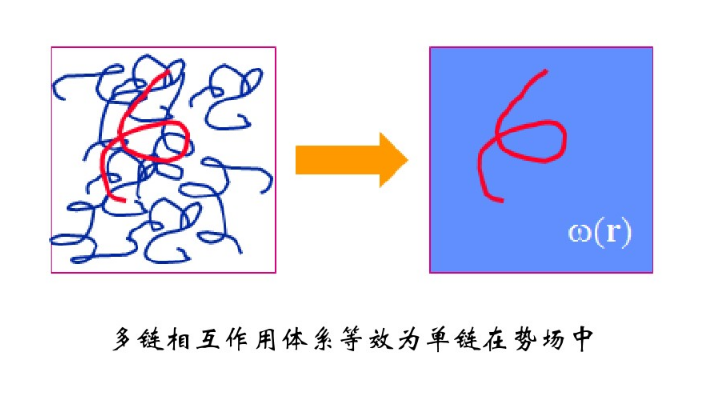
\includegraphics[scale=0.5]{./figures/Figure_22.png}
\end{figure}
自洽场模型是基于平均场近似的粗粒化模型,特别适合研究发生相分离的非均相高分子体系在平衡态的相结构及相图。
\begin{figure}[H]
\centering
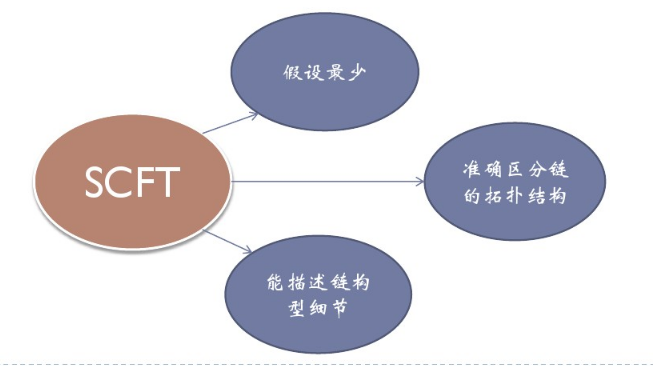
\includegraphics[scale=0.5]{./figures/Figure_23.png}
\end{figure}
\subsection{2.共聚物及分类}
共聚物:由两种或更多单体发生聚合反应所形成的聚合物称为共聚物,与之对应的是只有一种单体聚合而成的均聚物。共聚物的结构中具有至少两种结构单元,结构单元之间以化学键连接。由于共聚物包含至少两种结构单元,它可以根据其结构单元的排列顺序分成四种共聚物,图 2给出了当结构单元为A和B时的情况:依次为均聚物、交替共聚物、无规共聚物、嵌段共聚物和接枝共聚物。
\begin{figure}[H]
\centering
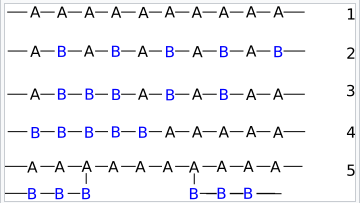
\includegraphics[scale=0.5]{./figures/Figure_25.png}
\caption{}
\end{figure}
\begin{itemize}
\item 交替共聚物:共聚物中两结构单元A和B严格交替相间,两者在共聚物中的摩尔分数均约为$50\%$
\item 无规共聚物:共聚物中两结构单元A和B随机出现,其中A和B自身连续的单元数不多,一般在几个到十几个。从统计上看,无规共聚物的某结构单元在聚合链上一段的含量等于其在整个聚合物中的含量。
\item 嵌段共聚物:由较长的只有结构单元A的链段和较长的只有结构单元B的链段构成,其中每一链段可达到几百到几千结构单元。
\item 接枝共聚物:接枝共聚物在结构上属于支化聚合物,其不仅有主链,还有较长的支链,且主链和支链是由不同种结构单元组成,如上图,主链全部是结构单元A,而支链全部是结构单元B。有时候,接枝聚合物的主链和支链可能都是共聚物,比如主链是A和B的无规共聚物,支链是A和B的交替共聚物,整体仍然是接枝共聚物。
\end{itemize}
\subsection{3.相分离}
嵌段聚合物在一定温度下会发生相分离现象,但一般的相分离体系如水和油,油滴的尺寸在微米尺度,而嵌段聚合物的嵌段间有化学键的链接,形成的相结构只有几十到几百纳米,所以被称为微相分离。嵌段共聚物的相转变温度主要取决于几个参数,总聚合物$N$,拓扑结构参数$n$,某嵌段所占的体积分数$f$和嵌段之间的Flory-Huggins相互作用参数$\chi$。随着嵌段所占的体积分数不同,嵌段聚合物相分离后形成的相结构也不同,有球状相,六方柱状相,层状相和双连续回转状相等结构。
\subsection{4.两嵌段柔性链共聚物体系}
首先给出两嵌段共聚物体系的连续高分子链的模型
\begin{figure}[H]
\centering
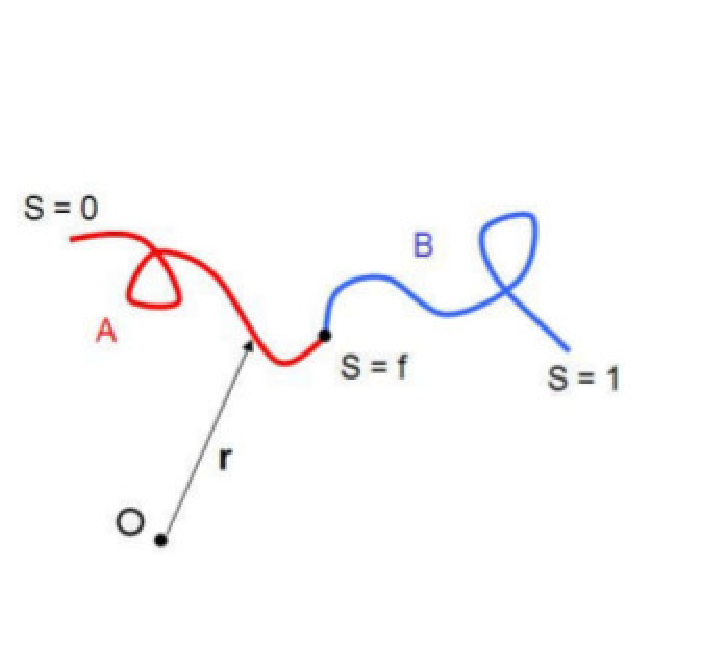
\includegraphics[scale=0.5]{./figures/dblock.pdf}
\caption{}
\end{figure}
我们考虑一般曲面上的两嵌段共聚物体系,假设系统有$n$个共聚物分子,每个共聚物分子是由$A$和$B$两类单体构成的两嵌段共聚物,它们限制在总面积为$S$的曲面上.单体$A$、$B$的体积分数分别为$f$和$1-f$,在平均场理论下,该系统的哈密顿量是
\begin{equation*}
H[w_+,w_-]=\frac{1}{\left|S\right|}\int\mathrm{d}x\left\{-w_+(x)+\frac{w_-^2(x)}{\chi N}\right\}-logQ[w_+(x),w_-(x)]\quad(1)
\end{equation*}
方程(1)中$w_-(x)$和$w_+(x)$是对应系统的场函数,其中$x$表示空间曲面上的点,$Q$是单链配分函数,$S$是曲面的面积,$\chi N$是体系参数,其中$\chi$是相互作用参数,$N$是聚合度.自由能函数关于场的一阶变分推导出下面的自洽场方程
\begin{equation*}
\begin{aligned}
\frac{\delta H}{\delta w_+(x)}&=\phi_A(x)+\phi_B(x)-1=0\\
\frac{\delta H}{\delta w_-(x)}&=\frac{2w_-(x)}{\chi N}-[\phi_A(x)-\phi_B(x)]=0
\end{aligned}
\end{equation*}
其中$\phi_A(x)$和$\phi_B(x)$是单体$A$和单体$B$的密度函数.然后结合连续高分子链的模型,得到自洽场系统.
\begin{equation*}
\begin{aligned}
\frac{\partial}{\partial s}q(x,s)&=\nabla_S^2q(x,s)-w(x,s)q(x,s),\quad q(x,0)=1\quad(2)\\
\frac{\partial}{\partial s}q^{\dagger}(x,s)&=-\nabla_S^2q^{\dagger}(x,s)+w(x,s)q^{\dagger}(x,s),\quad q^{\dagger}(x,1)=1\quad(3)\\
&w(x,s)=
\begin{cases}
w_+(x) - w_-(x) & 0\le s\le f\\
w_+(x) + w_-(x) & f\le s\le 1
\end{cases}
\end{aligned}
\end{equation*}
\begin{equation*}
\begin{aligned}
&Q=\frac{1}{\left|S\right|}\int\mathrm{d}xq(x,s)q^{\dagger}(x,1-s),\quad\forall s\in[0,1]\quad(4)\\
&\phi_A(x)=\frac{1}{Q}\int_0^f\mathrm{d}sq(x,s)q^{\dagger}(x,1-s)\quad(5)\\
&\phi_B(x)=\frac{1}{Q}\int_f^1\mathrm{d}sq(x,s)q^{\dagger}(x,1-s)\quad(6)
\end{aligned}
\end{equation*}
在系统中,正向传播子$q(x,s)(s:0\rightarrow 1)$表示长度为$s$的链在空间曲面位置$x$处的概率密度分布函数,其中变量$s$用于参数化每条共聚物链,$s=0$表示单体$A$的起始位置,$s=f$是单体$A$和单体$B$之间的连接点,反向传播子$q^{\dagger}(x,s)(s:1\rightarrow 0)$表示长度为$s$的链在空间曲面位置$x$处的概率密度分布函数.
\subsection{5.PDE Solver}
这里只给出正向传播子方程(2)的离散化,反向传播子方程(3)可以类似的得出.首先,给出(2)的变分形式
对$q\in H^1(S)$,满足
\begin{equation*}
\left(\frac{\partial}{\partial s}q,v\right)_S=-(\nabla_Sq,\nabla v)_S-(wq,v)_S,~~\text{ for all } v\in H^1(S).
\end{equation*}
其中$(\cdot,\cdot)_S$表示在曲面$S$上$L^2$内积.

找到$V_h\subset H^1(S)$得到(2)线性曲面有限元的离散形式,对$q_h=\sum\limits_{i=1}^Nq_i(s)\varphi_i(x)$,满足
\begin{equation*}
\left(\frac{\partial}{\partial s}q_h,v_h\right)_{S_h}=-(\nabla_{S_h}q_h,\nabla_{S_h} v_h)_{S_h}-(w_hq_h,v_h)_{S_h},~~\text{ for all } v_h\in H^1(S)\quad(4).
\end{equation*}

其中$(\cdot,\cdot)_{S_h}$表示在曲面$S_h$上$L^2$内积.$w_h(x,s)=\sum\limits_{i=1}^Nw(x_i,s)\varphi_i(x)$是$w(x,s)$的线性插值.得到方程(4)的半离散矩阵形式
\begin{equation*}
M\frac{\partial}{\partial s}\boldsymbol{q}(s)=-(A+F)\boldsymbol{q}(s)\quad(5)
\end{equation*}

其中
\begin{equation*}
\boldsymbol{q}(s)=(q_1(s),q_2(s),\cdots,q_N(s))^T
\end{equation*}

且
\begin{equation*}
M_{i,j}=(\varphi_i,\varphi_j),\quad A_{i,j}=(\nabla_S\varphi_i,\nabla_S\varphi_j),\quad F_{i,j}=(w_h\varphi_i,\varphi_j)
\end{equation*}

接下来,在$s-$方向使用Crank-Nicolson格式
\begin{equation*}
M\frac{\boldsymbol{q}^{n+1}-\boldsymbol{q}^n}{ds}=-\frac{1}{2}(A+F)\left[\boldsymbol{q}^{n+1}+\boldsymbol{q}^n\right]
\end{equation*}
$ds$是时间步长,整理得全离散的矩阵形式为
\begin{equation*}
\left[M+\frac{ds}{2}(A+F)\right]\boldsymbol{q}^{n+1}=\left[-\frac{ds}{2}(A+F)+M\right]\boldsymbol{q}^n
\end{equation*}

$s-$方向上的积分格式
\begin{equation*}
\int_0^{n_s}\mathrm{d}tf(s)=\Delta s\left\{-\frac{5}{8}(f_0+f_{n_s})+\frac{1}{6}(f_1+f_{{n_s}-1})-\frac{1}{24}(f_2+f_{{n_s}-2})+\sum\limits_{j=0}^{n_s}f_j\right\}
\end{equation*}
\subsection{6.自洽场迭代}
这里我们采用梯度下降法达到鞍点,具体而言,我们引入虚拟时间$t$并且在每个时间步,我们给出相应的鞍点搜索表达式
\begin{equation*}
\begin{aligned}
&\frac{\partial}{\partial t}w_+(x,t)=\frac{\delta H[w_+,w_-]}{\delta w_+(x,t)}\quad(7)\\
&\frac{\partial}{\partial t}w_-(x,t)=\frac{\delta H[w_+,w_-]}{\delta w_-(x,t)}\quad(8)
\end{aligned}
\end{equation*}
显然,当(2)和(3)达到平衡态时满足(7)和(8)

寻找SCFT的鞍点需要迭代方法,在SCFT的标准框架下,我们通过如下的迭代方案来更新$w_+(x), w_-(x)$.

step 1 给定初始估计的场$w_+(x), w_-(x)$.

step 2 计算在一般曲面上的正向传播子$q(x,s)$和反向传播子$q^{\dagger}(x,s)$.

step 3 由计算的$q(x,s)$和$q^{\dagger}(x,s)$通过自洽场系统得到$Q$,$\phi_A(x)$和$\phi_B(x)$,并计算出哈密顿量$H$.

step 4 对(2)和(3)使用迭代方法更新场$w_+(x,t)$和$w_-(x,t)$.

step 5 重复步骤 2-4 ,直到达到收敛标准.
\newpage
\section{自适应网格加密}
\subsection{1.网格数据结构}
以一个三角形网格为例,如下图
\begin{figure}[H]
\centering
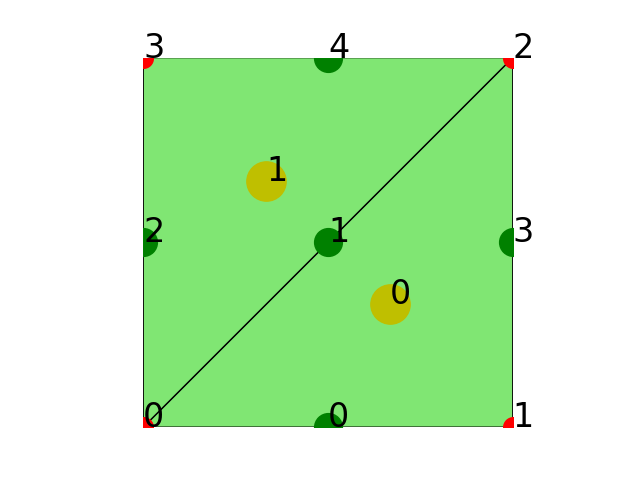
\includegraphics[scale=0.5]{./figures/picture_2.png}
\caption{}
\end{figure}
\begin{enumerate}
\item 边数组 `edge`
\begin{enumerate}
    \item 二维 $NE\times 2$ 数组 
    \item `edge[i, 0]` 和 `edge[i, 1]` 分别存储第 $i$ 条边的起点和终点的全局编号
    \item 如果第 $i$ 条边是边界边, 则规定从 `edge[i, 0]` 看向 `edge[i, 1]`, 网格区域一定在左手边
\end{enumerate}
\begin{lstlisting}
array([[0, 1],
       [2, 0],
       [3, 0],
       [1, 2],
       [2, 3])
\end{lstlisting}
\item 边与单元的相邻关系数组 `edge2cell`
\begin{enumerate}
    \item 二维 $NE \times 4 $ 的数组
    \item `edge2cell[i, 0]` 和 `edge2cell[i, 1]` 分别存储第 $i$ 条边左右两个单元的全局编号
\newpage
    \item `edge2cell[i, 2]` 和 `edge2cell[i, 3]` 分别存储第 $i$ 条边在左右两个单元中的局部编号
    \item 如果是边界边, 则
\begin{enumerate}
        \item `edge2cell[i, 0] = edge2cell[i, 1]` 
        \item `edge2cell[i, 2] = edge2cell[i, 3]`
\end{enumerate}
\end{enumerate}
\begin{lstlisting}
array([[0, 0, 1, 1],
       [0, 1, 0, 0],
       [1, 1, 2, 2],
       [0, 0, 2, 2],
       [1, 1, 1, 1],)
\end{lstlisting}
\item 单元与单元的相邻关系数组`cell2cell`
\begin{enumerate}
  \item 二维 $NE \times 3$ 的数组
  \item `cell2cell[i, 0]` 和 `cell2cell[i, 1]` 和 `cell2cell[i, 2]`分别存储第 $i$ 个单元的邻居单元的全局编号,如果没有邻居单元,邻居单元的全局编号就是这个单元的全局编号.
  
\end{enumerate}
\begin{lstlisting}
array([[1, 0, 0],
       [0, 1, 1]])
\end{lstlisting}
\item 单元与边的关系`cell2edge`
\begin{enumerate}
\item 二维 $NC \times 3$ 的数组
\item `cell2edge[i, 0:3]`是存储第`i`个单元的逆时针对应边的全局编号
\end{enumerate}
\begin{lstlisting}
array([[ 1,  0,  3],
       [ 1,  4,  2]])
\end{lstlisting}
\end{enumerate}
\subsection{2.约定}
\begin{figure}[H]
\centering
\begin{minipage}[!htbp]{0.3\linewidth}
    \centerline{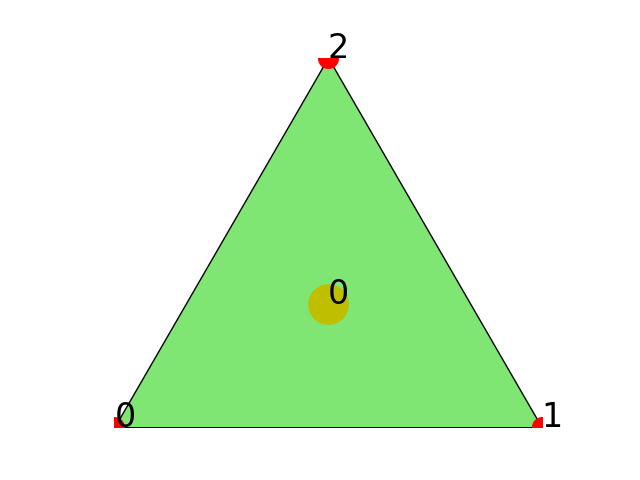
\includegraphics[width=6cm]{./figures/Figure_3.png}}
    \centerline{加密前}
\end{minipage}
\hspace{0.25in}		
\begin{minipage}[!htbp]{0.3\linewidth}
    \centerline{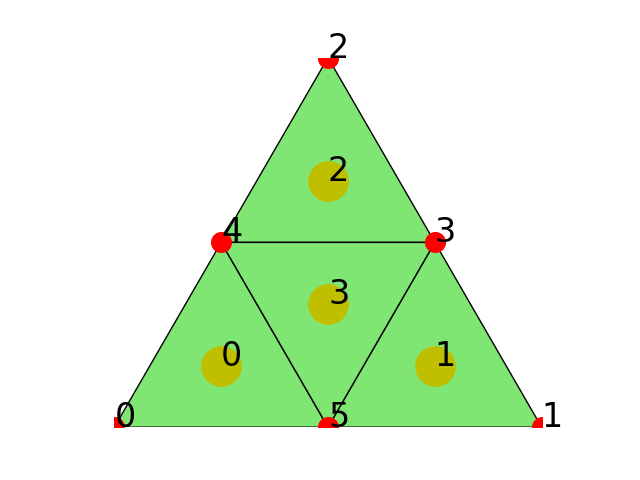
\includegraphics[width=6cm]{./figures/Figure_2.png}}
    \centerline{加密后}
\end{minipage}
\end{figure}
我们的加密方式是取三角形三条边的中点,然后把三条边的中点连起来,这样就把原来的三角形分成了四个小三角形,我们约定四个小三角形的局部编号顺序为0, 1, 2, 3.然后约定局部编号为3的三角形的顶点的局部编号的顺序和他父单元边的局部编号顺序一致.
\subsection{3.Tritree的数据结构}
\begin{enumerate}
\item 生成Tritree类的时候, 是从`TriangleMesh`中继承网格
\item 定义初始化时,需要继承的是网格点`node`, 单元`cell`, 根据`node`和`cell`初始化网格, 然后得到单元的个数`NC`, 再根据单元的个数生成两个数组`parent`和`child`, 这两个数组分别是值为 $-1$ 的 $NC \times 2$ 和 $NC \times 4$ 的数组
\item 定义叶子单元指标(即`leaf\_cell\_index`): 根据数组`child`的值为 $-1$ 的所有行维度的索引值`idx`, 返回叶子单元的`idx`.
\item 定义叶子单元(即`is\_leaf\_cell`): 是根据叶子单元指标`idx`来判断是否是叶子单元:若`idx`是`None`, 返回的是`child[:, 0]==-1`, 是布尔型数组, 表示的意思是第 $0$ 列的所有行的值等于 $-1$ 为真;若`idx`不是`None`则返回的是`child[idx, 0] == -1`, 是布尔型数组, 表示的意思是第 $0$ 列的所有对应`idx`的值等于 $-1$ 为真
\item 定义根单元(即`is\_root\_cell`): 是根据单元指标`idx`来判断是否是根单元: 若`idx`是`None`, 返回的是`parent[:, 0]==-1`, 是布尔型数组, 表示的意思是第 $0$ 列的所有行的值等于 $-1$ 为真; 若`idx`不是`None`则返回的是`parent[idx, 0] == -1`, 是布尔型数组, 表示的意思是第 $0$ 列的所有对应`idx`的值等于 $-1$ 为真
\end{enumerate}
\subsection{4.加密算法}
\begin{enumerate}
\item 定义加密(即`refine`): 传入的数据是标记`marker`(标记是自适应加密过程中必不可少的一步, 它构成自适应加密循环的过程,自适应加密过程为: 求解 $\to$ 估计 $\to$ 标记 $\to$ 加密或放粗). 对于传入的数据`marker`若`marker == None`为真, 指标的索引`idx`就是叶子单元的索引, 否则, 叶子单元指标`idx`就是标记之后的索引. 若`idx`是`None`则返回`False`, 加密结束, 
如果`idx`的长度大于 $0$, 则进行如下,我们定义`isMarkedCell`是长度为`NC`的布尔型数组,然后把`isMarkedCell`索引中`idx`是叶子单元的等于`True`.
\item 扩展标记单元
\begin{figure}[H]
\centering
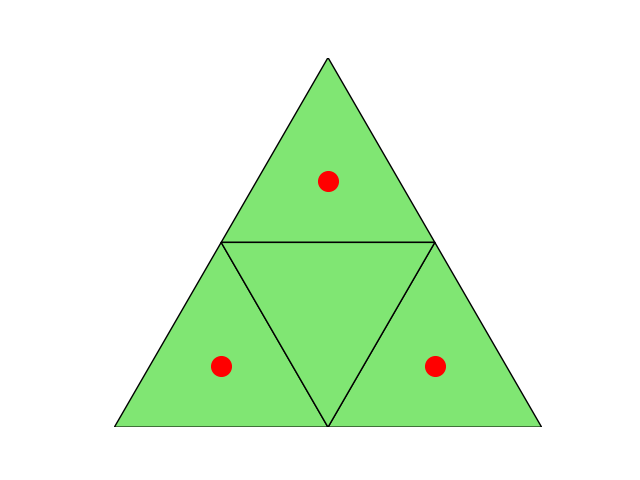
\includegraphics[scale=0.5]{./figures/Figure_8.png}
\caption{}
\end{figure}
case 1:如图 5,如果这个单元是叶子单元但不是被标记的单元,但是这个单元的邻居单元至少有两个以上的单元是被标记的单元或者不是叶子单元,那么这个单元也应该被标记.
\begin{figure}[H]
\centering
\begin{minipage}[!htbp]{0.3\linewidth}
    \centerline{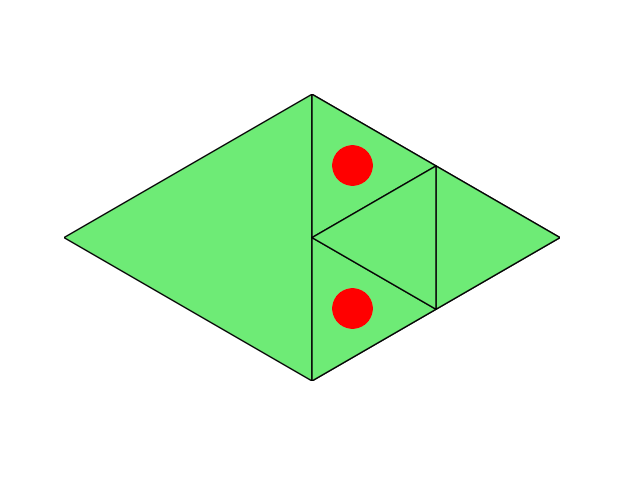
\includegraphics[width=6cm]{./figures/Figure_4.png}}
    \centerline{(a)}
\end{minipage}
\hspace{0.25in}		
\begin{minipage}[!htbp]{0.3\linewidth}
    \centerline{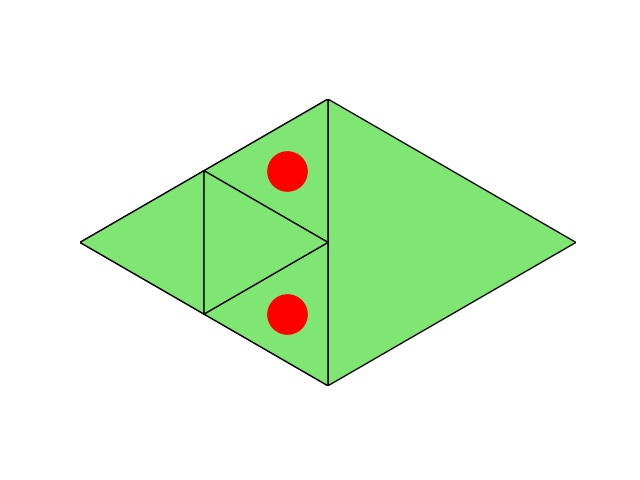
\includegraphics[width=6cm]{./figures/Figure_5.png}}
    \centerline{(b)}
\end{minipage}
\caption{}
\end{figure}
case 2:如图 6(a)它的左边单元是叶子单元但不是被标记的单元,右边单元不是叶子单元,但是右边单元中与左边单元相邻的孩子单元是被标记的单元,那么左边单元也应该被标记.\\
如图 6(b)它的右边单元是叶子单元但不是被标记的单元,左边单元不是叶子单元,但是左边单元中与右边单元相邻的孩子单元是被标记的单元,那么右边单元也应该被标记.\\
扩展单元的时候我们找到是上面两种情况的叶子单元,把`isMarkedCell`索引中`idx`是上面两种情况的叶子单元的等于`True`,现在我们就找到了所有要被加密的单元.
\item 找到加密的边和`edge2newNode`\\
我们定义`refineFalg`是长度为`NE`的布尔型数组,通过`cell2edge`找到`isMarkedCell`的边,然后把`refineFalg`中索引是这些边的等于`True`,但是这里要除去左边是叶子单元,右边不是叶子单元或者左边不是叶子单元边,右边是叶子单元的那些边,在`refineFalg`索引是这些边的等于`False`,要加密边的总数为`NNN=refineFalg.sum()`.\\
`edge2newNode`是长度为`NE`的数组,加密之后边上的新的点的编号为`NN+np.arange(NNN)`.
\item 加密成四个小三角形\\
首先`NCC`是标记单元的个数, 再根据标记单元的个数生成`cell4`是值为0的`4*NC`$\times$3数组和`parent4`,`child4`分别是值为 $-1$ 的`4*NC`$\times$2 和`4*NC`$\times$4的数组,然后找到一分为四的每个小三角形的顶点,然后把连起来,最后把所有的`node`,`cell`,`parent`,`child`拼到一起.
\begin{figure}[H]
\centering
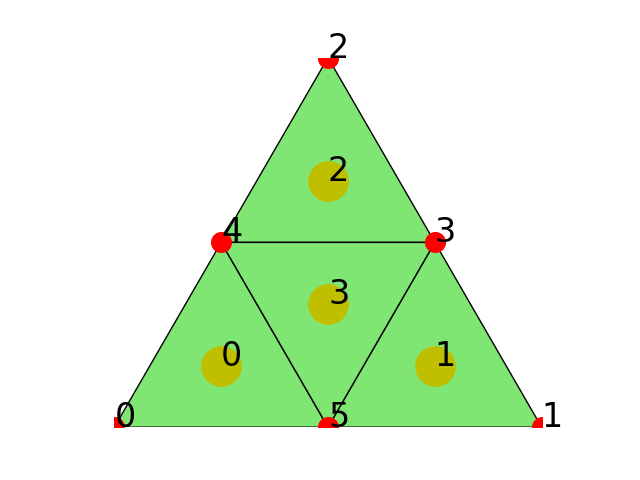
\includegraphics[scale=0.5]{./figures/Figure_2.png}
\caption{}
\end{figure}
\begin{lstlisting}
cell4[:NCC, 0] = cell[isMarkedCell, 0] 
cell4[:NCC, 1] = edge2newNode[cell2edge[isMarkedCell, 2]] 
cell4[:NCC, 2] = edge2newNode[cell2edge[isMarkedCell, 1]] 
parent4[:NCC, 0] = idx 
parent4[:NCC, 1] = 0
self.child[idx, 0] = NC + np.arange(0, NCC)
\end{lstlisting}
\item 生成协调化网格
\begin{figure}[H]
\centering
\begin{minipage}[!htbp]{0.3\linewidth}
    \centerline{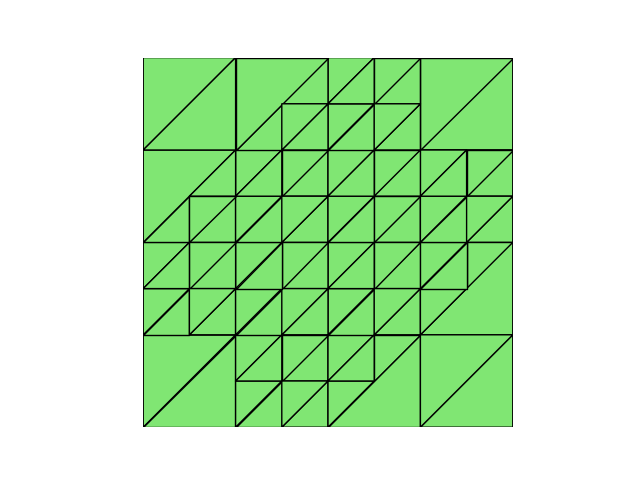
\includegraphics[width=6cm]{./figures/Figure_9.png}}
    \centerline{协调化之前}
\end{minipage}
\hspace{0.25in}		
\begin{minipage}[!htbp]{0.3\linewidth}
    \centerline{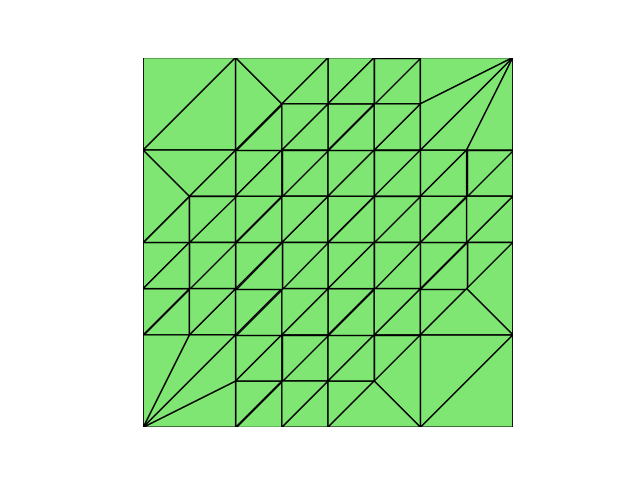
\includegraphics[width=6cm]{./figures/Figure_7.png}}
    \centerline{协调化之后}
\end{minipage}
\end{figure}
最后我们进行协调化处理,找到每条加密边的中点和对应单元的顶点把它们连在一起,这里要注意最后的`cell`的处理.\\
然后调用`TriangleMesh(node, cell)`,生成协调化网格`Tmesh`.
\end{enumerate}
例子1:加密圆穿过的单元
\begin{figure}[H]
\centering
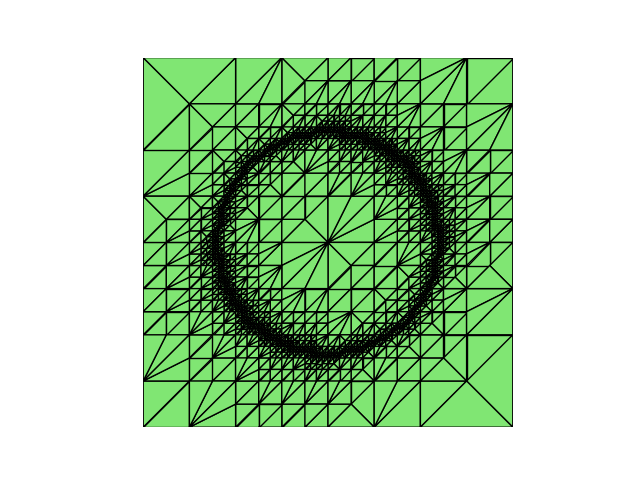
\includegraphics[scale=0.5]{./figures/Figure_12.png}
\caption{}
\end{figure}
例子2:球面上的加密
\begin{figure}[H]
\centering
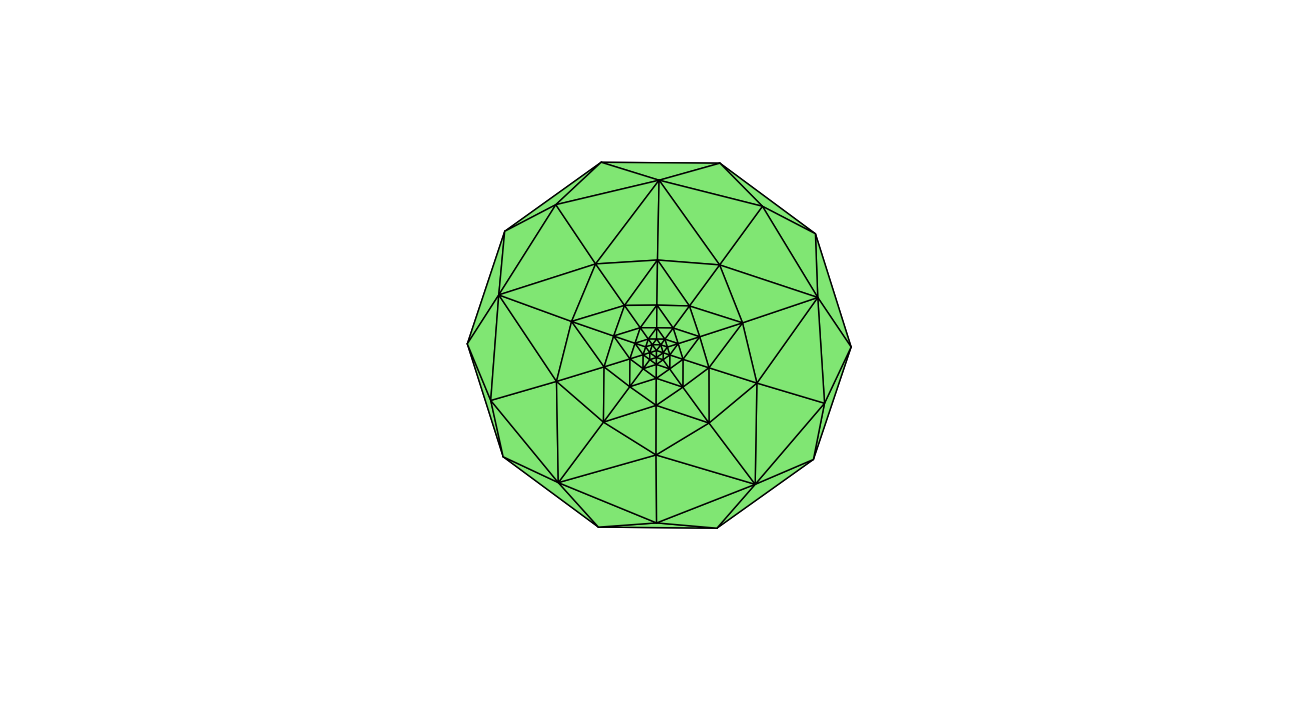
\includegraphics[scale=0.5]{./figures/Figure_11.png}
\caption{}
\end{figure}
\newpage
\section{自适应有限元方法}
\subsection{1.预备知识}
由有限元方法的先验误差估计知,虽然求得了数值解,但不能知道误差的具体大小,特别是当解具有奇性的时候,要得到好的数值解要求网格尺寸$h$足够小,这是不现实的。自适应有限元方法(AFEM)是求解科学计算和工程问题的最有效方法之一,特别对存在奇性或者多尺度性质的问题有很强的适定性。它根据计算结果和已知量自动控制计算的过程,逐步调整网格,使得误差分布得比较均匀,从而以尽量少的计算量达到所要求的精度,提高计算效率。自适应方法的研究对象是连续的微分或者积分方程,其基本算法包含两步:当前离散空间上的求解和调整后的离散空间上的校正。自适应算法奏效的基本条件是:后验误差估计子的可靠性和有效性,调整后的离散空间能够捕捉到足够的局部高频信息。后验误差估计子是基于近似解和其他已知条件的一个可计算量,它既是真实误差的一个上界又是真实误差的一个下界。后验误差估计子是调整离散空间的基础。调整离散空间是自适应方法至关重要的部分,目前科学工程计算中调整离散空间的方法有h-方法、p-方法、hp-方法和r-方法。h-方法是一种局部网格加密方法,它保持单元多项式次数不变,通过逐步加密网格来调整离散空间,和h-方法不同,p-方法保持网格不变,通过提高单元多项式次数来调整离散空间。hp-方法是h-和p-方法的结合,即在加密网格的同时改变单元多项式的次数。r-方法是在不改变节点总数和多项式次数的前提下通过移动节点来调整离散空间。

自适应有限元算法流程图见图 10,由下面的几步操作构成:
\begin{center}
求解$\rightarrow$误差估计$\rightarrow$标记$\rightarrow$加密
\end{center}
\begin{itemize} 
\item 求解:在当前网格上求得数值解$u_h$;包括计算刚度矩阵和载荷向量,求解代数方程组.
\item 误差估计:根据后验误差估计,由已知数据和数值解$u_h$估计单元误差和全局误差.
\item 标记:根据标记策略和计算的单元误差,对网格中需要加密的单元进行标记.
\item 加密:依据加密算法,对标记的单元进行加密,得到新网格.
\end{itemize}
\begin{figure}[H]
\centering
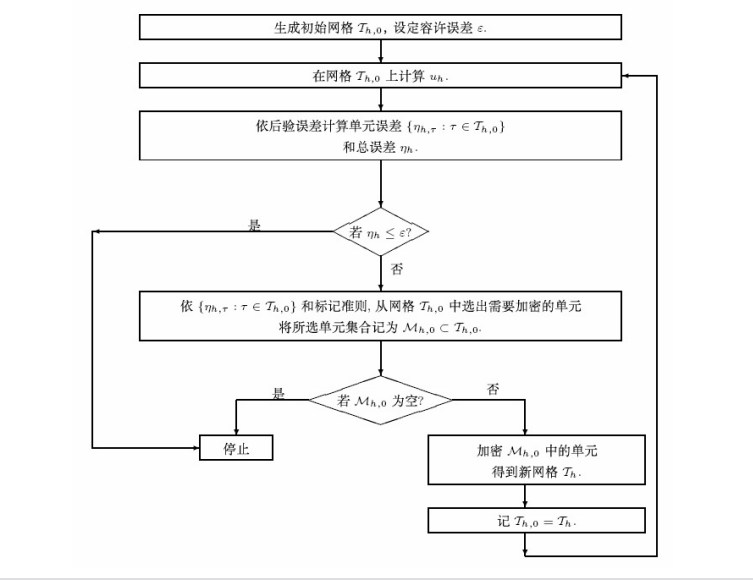
\includegraphics[scale=0.6]{./figures/Figure_13.png}
\caption{}
\end{figure}
\subsection{2.后验误差估计}
后验误差估计是自适应有限元方法中重要的一部分,它是根据数值解和已知数据构造单元估计子$\{\eta_{\tau}:\tau\in\mathcal{T}_h\}$和全局估计子$\eta_h^2=\sum\limits_{\tau\in\mathcal{T}_h}\eta_{\tau}^2$,来局部和全局的估计误差$e_h=u-u_h$.一个好的后验误差估计既是误差的下界也是误差的上界,即
\begin{equation*}
C_1\eta_h\le\left\|\left|e_h\right|\right\|\le C_2\eta_h
\end{equation*}
上界保证了计算结果的准确性,下界则保证了计算结果的有效性。特别地,$\frac{\eta_h}{\left\|\left|e_h\right|\right\|}\rightarrow 1$,则称后验误差估计是渐进准确的。$\eta_h$用来控制自适应算法的终止,单元误差估计子则表现了误差的分布情况。

后验误差估计主要可归为两类:残量型后验误差估计和重构型后验误差估计。残量型后验误差估计是通过计算局部残量而得到误差估计。对残量的估计方式可分为显式法和隐式法,导出的后验误差估计分别称为显式后验误差估计和隐式后验误差估计。重构型误差估计具有与问题(方程)无关、与有限元形式无关等优点,且实现简单、计算量小、具有鲁棒性(是指控制系统在一定(结构,大小)的参数摄动下,维持其它某些性能的特性)。重构型后验误差估计是基于后处理技术的误差估计,后处理是在得到数值解后,通过少量的计算,来改善有限元解的质量。常用的后处理的方法有:加权平均、插值后处理、最小二乘法、局部或全局投影等。用后处理的解代替真解,它可用来估计真实误差。
\subsection{3.基于WAR的后验误差估计}
\begin{figure}[H]
\centering
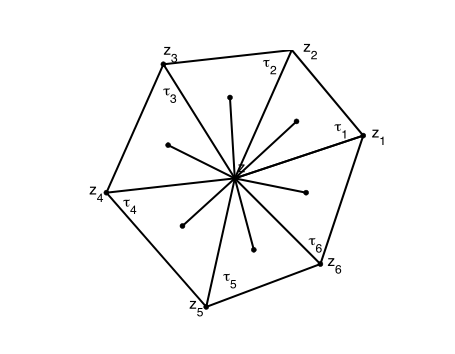
\includegraphics[scale=0.5]{./figures/Figure_24.png}
\caption{}
\end{figure}
首先我们给出三角形单元的五种加权平均格式的定义。记$\mathcal{T}_h$为区域$\Omega\subset\mathbb{R}^2$的三角剖分,$S_h$为$\mathcal{T}_h$上对应的线性元空间
\begin{equation*}
S_h=\{v\in H^1(\Omega):v \in P_1(\tau),\forall\tau\in\mathcal{T}_h\}
\end{equation*}
其中$P_k(D)$表示$D\in\mathbb{R}^2$上次数不超过$k$次的多项式集合。对任一内节点$z$,记$\mathcal{K}_z$为点$z$的单元片。如图 11,设$\tau_1,\tau_2,\cdots,\tau_m\in \mathcal{T}_h$为单元片$\mathcal{K}_z$中的单元,记$c_i$为单元$\tau_i$的重心,$S_i$为单元$\tau_i$的面积,$d_i=\left\|z-c_i\right\|$表示点$z$与$c_i$的距离,$\alpha_i$为三角形$\tau_i$中以$z$顶点的角的角度。对有限元函数$v\in S_h$,定义加权平均格式如下:

简单平均:
\begin{equation*}
S_hv(z):=\sum\limits_{i=1}^m\frac{1}{m}\nabla v\big|_{\tau_i}
\end{equation*}

面积平均
\begin{equation*}
G_hv(z):=\sum\limits_{i=1}^m\frac{S_i}{\sum\limits_{j=1}^mS_j}\nabla v\big|_{\tau_i}
\end{equation*}

面积调和平均
\begin{equation*}
H_hv(z):=\sum\limits_{i=1}^m\frac{\frac{1}{S_i}}{\sum\limits_{j=1}^m\frac{1}{S_j}}\nabla v\big|_{\tau_i}
\end{equation*}

角度平均
\begin{equation*}
A_hv(z):=\sum\limits_{i=1}^m\frac{\alpha_i}{\sum\limits_{j=1}^m\alpha_j}\nabla v\big|_{\tau_i}
\end{equation*}

距离调和平均
\begin{equation*}
D_hv(z):=\sum\limits_{i=1}^m\frac{\frac{1}{d_i}}{\sum\limits_{j=1}^m\frac{1}{d_j}}\nabla v\big|_{\tau_i}
\end{equation*}

上面我们讨论了梯度重构的加权平均方法,加权平均方法是一种简单的后处理方法,基于加权平均方法可以获得有效的后验误差估计,因此在自适应方法中被广泛的应用。基于加权平均方法的后验误差估计具有如下形式:
\begin{equation*}
\eta_a=\left\|R_hu_h-\nabla u_h\right\|_{0,\Omega},\quad R_hu_h(z)=\sum\limits_{j=1}^{m}\nabla u_h(z_j)\omega_j
\end{equation*}
其中,$R_h$表示加权平均算子,$z_j$为样本点,$z$为重构点,$\omega_j$为权函数。我们考虑基于前面讨论的加权平均方法的后验误差估计。记$S_h,G_h,H_h,A_h,D_h$分别表示简单平均算子、面积平均算子、面积调和平均算子、角度平均算子和距离调和平均算子,我们记
\begin{equation*}
\eta_{S,\tau}^2=\left\|S_hu_h-\nabla u_h\right\|_{0,\tau}^2,\qquad\eta_S^2=\sum\limits_{\tau\in\mathcal{T}_h}\eta_{S,\tau}^2
\end{equation*}
\begin{equation*}
\eta_{G,\tau}^2=\left\|G_hu_h-\nabla u_h\right\|_{0,\tau}^2,\qquad\eta_G^2=\sum\limits_{\tau\in\mathcal{T}_h}\eta_{G,\tau}^2
\end{equation*}
\begin{equation*}
\eta_{H,\tau}^2=\left\|H_hu_h-\nabla u_h\right\|_{0,\tau}^2,\qquad\eta_H^2=\sum\limits_{\tau\in\mathcal{T}_h}\eta_{H,\tau}^2
\end{equation*}
\begin{equation*}
\eta_{A,\tau}^2=\left\|A_hu_h-\nabla u_h\right\|_{0,\tau}^2,\qquad\eta_A^2=\sum\limits_{\tau\in\mathcal{T}_h}\eta_{A,\tau}^2
\end{equation*}
\begin{equation*}
\eta_{D,\tau}^2=\left\|D_hu_h-\nabla u_h\right\|_{0,\tau}^2,\qquad\eta_D^2=\sum\limits_{\tau\in\mathcal{T}_h}\eta_{D,\tau}^2
\end{equation*}




\nocite{*}
\bibliography{}
\end{document}


